\begin{table}[t]
\centering
\caption{Eighty-nine-item-per-task LongBench v2 pilot results for \RunModel. Quality is exact-match accuracy, and retrieval-augmented generation (RAG) denotes the episodic retrieval baseline.}
\label{tab:main_89item_results}
\resizebox{\textwidth}{!}{%
\begin{tabular}{lccccc|ccccc}
\toprule
& \multicolumn{5}{c|}{Quality} & \multicolumn{5}{c}{Violation rate} \\
Strategy & 2K & 4K & 8K & 16K & 32K & 2K & 4K & 8K & 16K & 32K \\
\midrule
Truncation & 0.29 & 0.27 & 0.27 & 0.33 & 0.33 & 0.00 & 0.00 & 0.00 & 0.00 & 0.00 \\
Summary & 0.30 & 0.24 & 0.26 & 0.29 & 0.31 & 0.03 & 0.07 & 0.05 & 0.07 & 0.03 \\
RAG & 0.30 & 0.31 & 0.35 & 0.34 & 0.31 & 0.00 & 0.00 & 0.00 & 0.00 & 0.00 \\
\bottomrule
\end{tabular}%
}
\end{table}

\begin{table}[t]
\centering
\caption{SWE-bench Verified scaffold diagnostic for the same 89-item-per-task run. Retrieval-augmented generation (RAG) denotes the episodic retrieval baseline. The SWE value is a patch-similarity proxy, not official SWE-bench accuracy. Repeated high-budget cells remain collapsed because these SWE prompts are short enough that the effective strategy inputs become identical at 8K and above.}
\label{tab:swe_proxy_diagnostic}
\resizebox{\textwidth}{!}{%
\begin{tabular}{llcccc}
\toprule
Strategy & Budget regime & SWE proxy & Violation rate & Mean used tokens & Max peak tokens \\
\midrule
Truncation & 2K & 0.18 & 0.00 & 561 & 1,973 \\
Truncation & 4K & 0.19 & 0.00 & 646 & 3,299 \\
Summary & 2K & 0.18 & 0.00 & 570 & 1,973 \\
Summary & 4K & 0.19 & 0.00 & 650 & 3,299 \\
RAG & 2K & 0.18 & 0.07 & 557 & 4,542 \\
RAG & 4K & 0.19 & 0.03 & 644 & 4,542 \\
All strategies & 8K--32K & 0.19 & 0.00 & 788 & 4,542 \\
\bottomrule
\end{tabular}%
}
\end{table}

\begin{figure}[t]
  \centering
  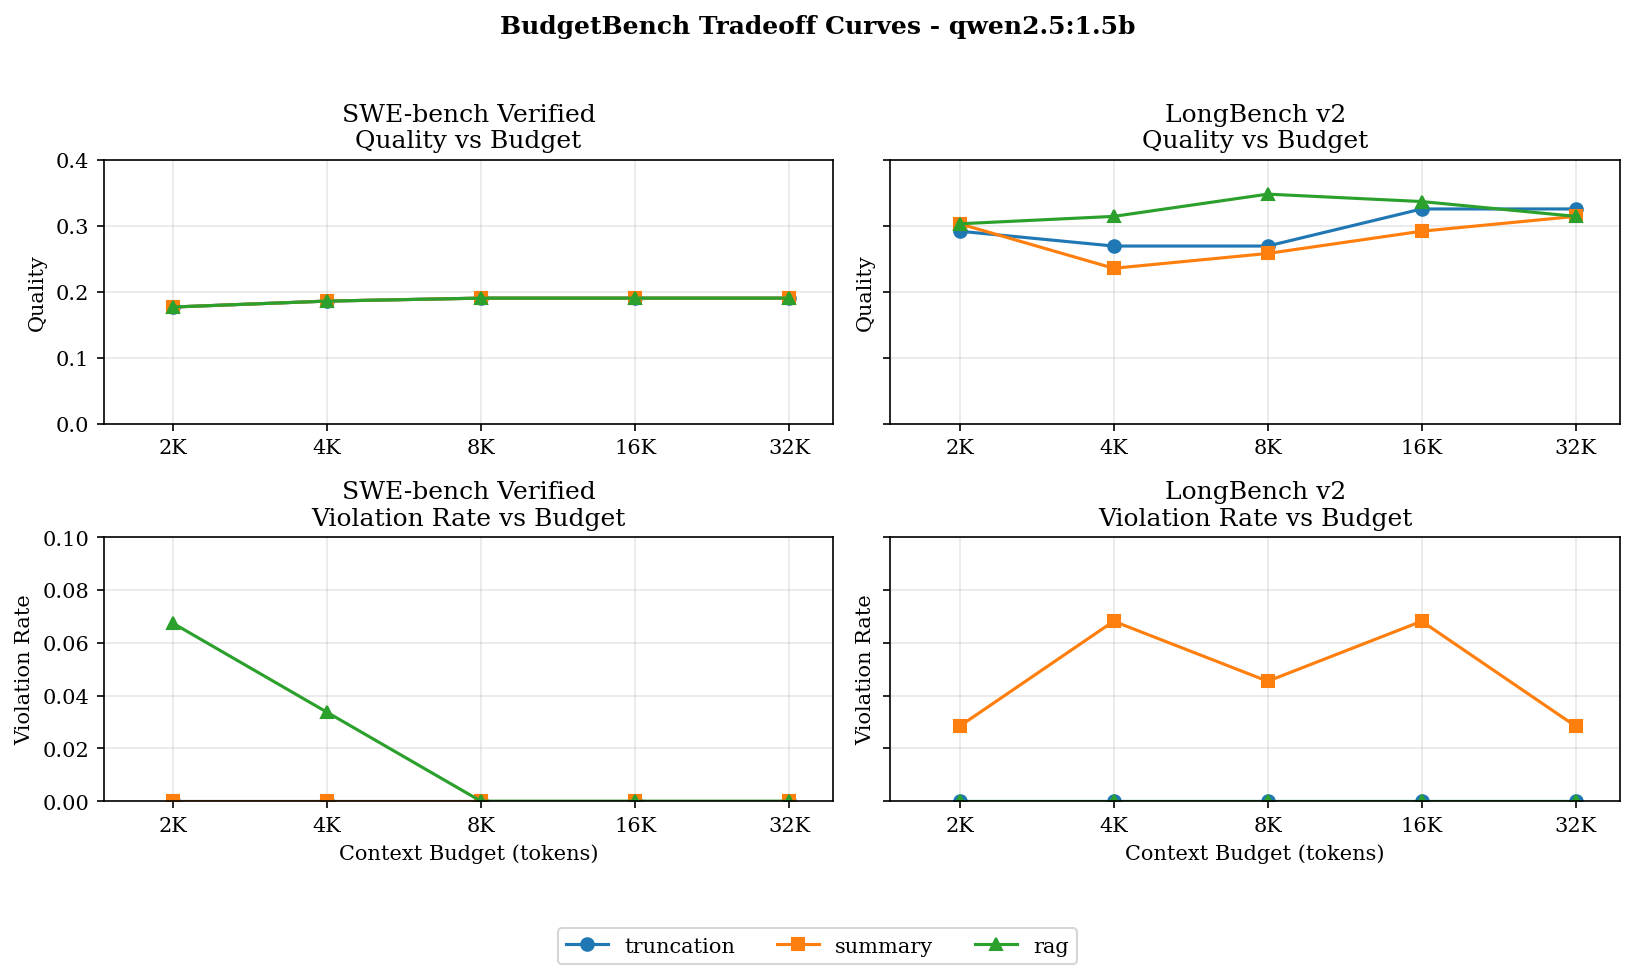
\includegraphics[width=\textwidth]{../results/figures/tradeoff_curves_qwen2_5_1_5b.png}
  \caption{Quality and budget-violation curves for the 89-item-per-task pilot run. Blue circles denote truncation, orange squares denote summary, and green triangles denote retrieval-augmented generation (RAG). SWE quality is the patch-similarity proxy; LongBench v2 quality is exact-match accuracy.}
  \label{fig:tradeoff_89item}
\end{figure}

\begin{figure}[t]
  \centering
  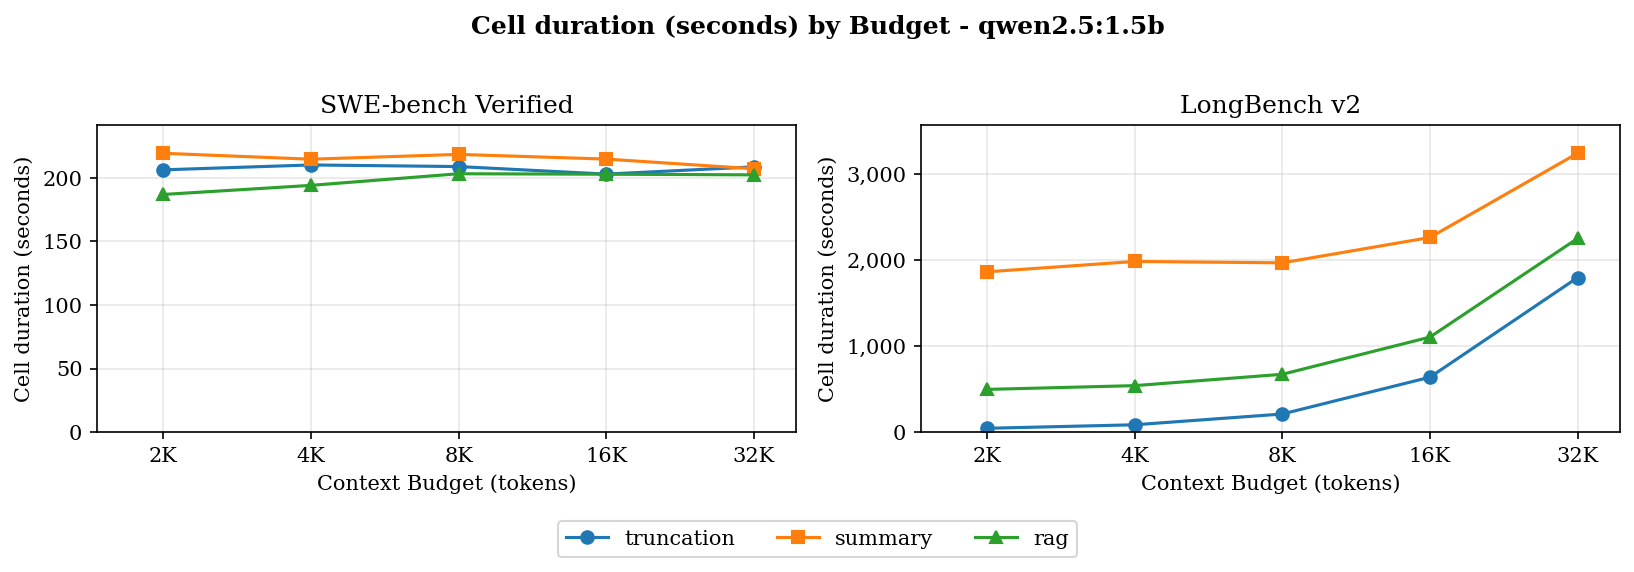
\includegraphics[width=\textwidth]{../results/figures/duration_curves_qwen2_5_1_5b.png}
  \caption{Cell-level runtime by task, strategy, and active context budget. Blue circles denote truncation, orange squares denote summary, and green triangles denote retrieval-augmented generation (RAG).}
  \label{fig:duration_89item}
\end{figure}

\begin{figure}[t]
  \centering
  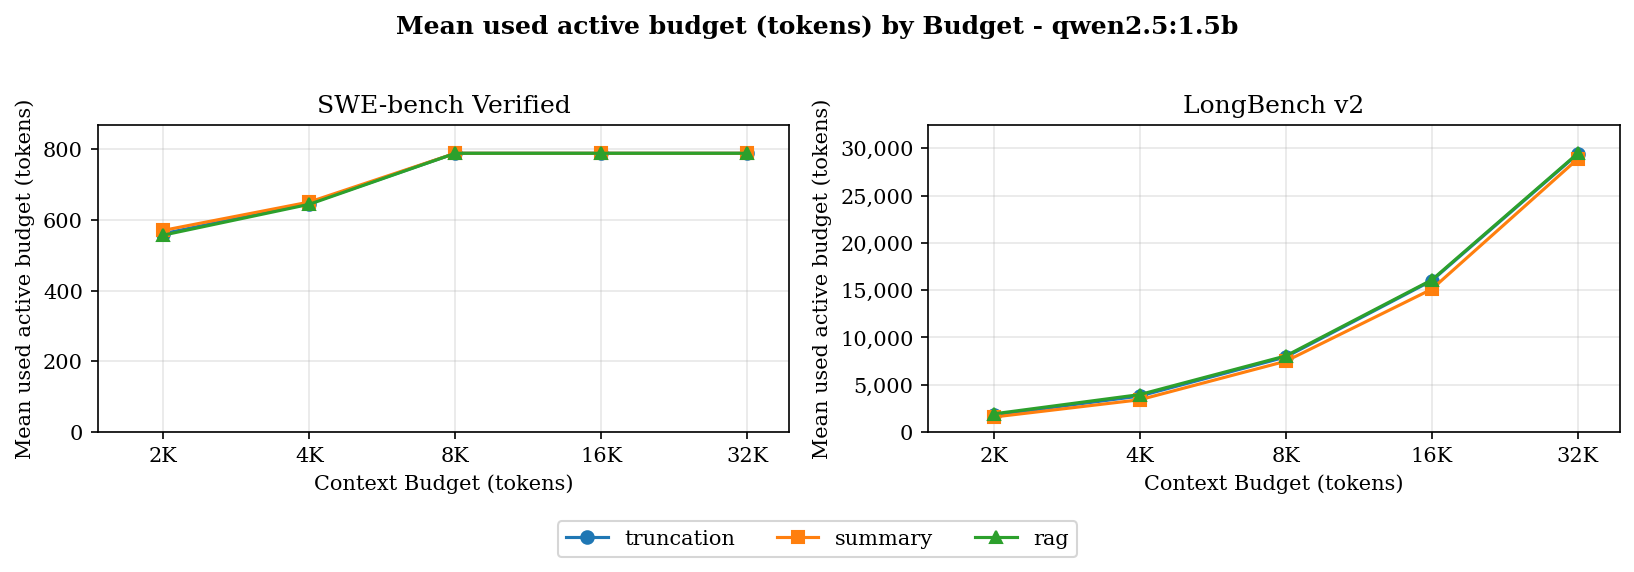
\includegraphics[width=\textwidth]{../results/figures/used_budget_curves_qwen2_5_1_5b.png}
  \caption{Mean used active budget by task, strategy, and tier. Blue circles denote truncation, orange squares denote summary, and green triangles denote retrieval-augmented generation (RAG).}
  \label{fig:used_budget_89item}
\end{figure}
